\chapter{Desarrollo de la solución propuesta}
\label{cap:descrip}

Como se ha introducido a lo largo del capítulo \ref{cap:introduccion}, para el correcto funcionamiento de la línea es necesario un operador que controle y supervise el funcionamiento de la misma, realice la carga de granza en la extrusora y la carga y descarga de los carretes en la bobinadora. Debido a ello se generan errores en la producción que sólo son visibles una vez que el producto ha sido almacenado y sometido a las convenientes pruebas de calidad, almacenando asi un producto que no es de la calidad necesaria para comercializarlo.\\

Para minimizar el error humano, se propone la implementación de un sistema de aquisición y procesamiento de datos (SCADA) que permita el análisis durante y después de la producción de los diferentes parámetros del sistema. Estos son el diámetro final del filamento, las temperaturas a lo largo de la extrusora y las velocidades de extrusión. De esta manera podemos ver los aspectos que influyen en el diámetro y que el propio sistema sea capaz de corregirlo en tiempo real durante la producción. El sistema que se desarrolle, deberá ser lo más ampliable que se pueda, de esa manera, será útil en casi cualquier línea de extrusión sin importar la instrumentación que se disponga.

\section{Planificación}
\label{sec:planificacion}

El proyecto está definido por dos fases:\\

La primera fase en la que se desarrollará el sistema de adquisición de datos constará de los siguientes puntos:

\begin{itemize}
    \item Recopilación y análisis de la documentación de todos los dispositivos de interés para el proyecto de la línea de extrusión.
    \item Defición de los requisitos respecto a comunicaciones necesarias entre los dispositivos de la línea y el sistema de adquisición.
    \item Determinar los requisitos del autómata progamable industrial (PLC) a utilizar.
    \item Programación del PLC. Puesto que será el encargado de llevar el control de la planta, deberemos programar la adquisición de datos para establecer el control sobre la linea.
\end{itemize}

En esta fase se pondrá en marcha todo el sistema en la planta, instalando el PLC y cableando toda la red de comunicaciones y sensores que disponemos. Así mismo se almacenarán datos de los seis sensores de temperatura que dispone la planta (cinco de ellos en extrusora y uno en bañera de enfriamiento) y el sensor de diámetro. Con los datos adquiridos se modelará parcialmente la planta para intentar hacer un control en lazo cerrado entre la unión tractora de filamento y el sensor de diámetro del mismo. Durante esta fase se diseñará un sistema, para poder visualizar los datos adquiridos de forma remota.\\

La segunda fase del proyecto consistirá en la implementación en planta de los distintos reguladores diseñados y probados en la fase anterior. Como primera aproximación la salida a controlar será el diámetro del filamento y la entrada la velocidad de tracción, ya que es la variable que influye directamente en el diámetro a conseguir. Se estudiarán los beneficios de usar distintos tipos de controladores como pueden ser PID, fuzzy, etc. para posteriormente estudiar los beneficios e inconvenientes de cada uno de ellos.\\

Para el completo desarrollo de esta segunda fase, y poder demostrar el correcto funcionamiento en la línea, necesitaremos la aprobación de la empresa pels que explota la línea de extrusión. Aunque se tratará de un sistema modular que será fácil de integrar en otras líneas de producción parecidas. Siendo el sistema totalmente compatible y escalable para futuras lineas de extrusión que se adquieran.\\

Los plazos asignadaos a cada una de las distintas fases que componen el proyecto, se puede ver en el Anexo \ref{ane:gant}

\section{Herramientas empleadas}
\label{sec:herramientas}

\subsection{GitHub}
GitHub es una plataforma de desarrollo colaborativo en el que se pueden alojar proyectos utilizando la herramienta de control de versiones Git. El código almacenado en esta plataforma es de dominio público, sin embargo también existe la posibilidad de crear repositorios privados creándonos una cuenta de pago.\\

Para la realización del proyecto se ha creado un repositorio online \cite{githubTFG} en el que se han ido subiendo todos los ficheros que se han ido utilizando para la realización del mismo (ver Figura \ref{fig:github}).

\begin{figure}[H]
    \centering
    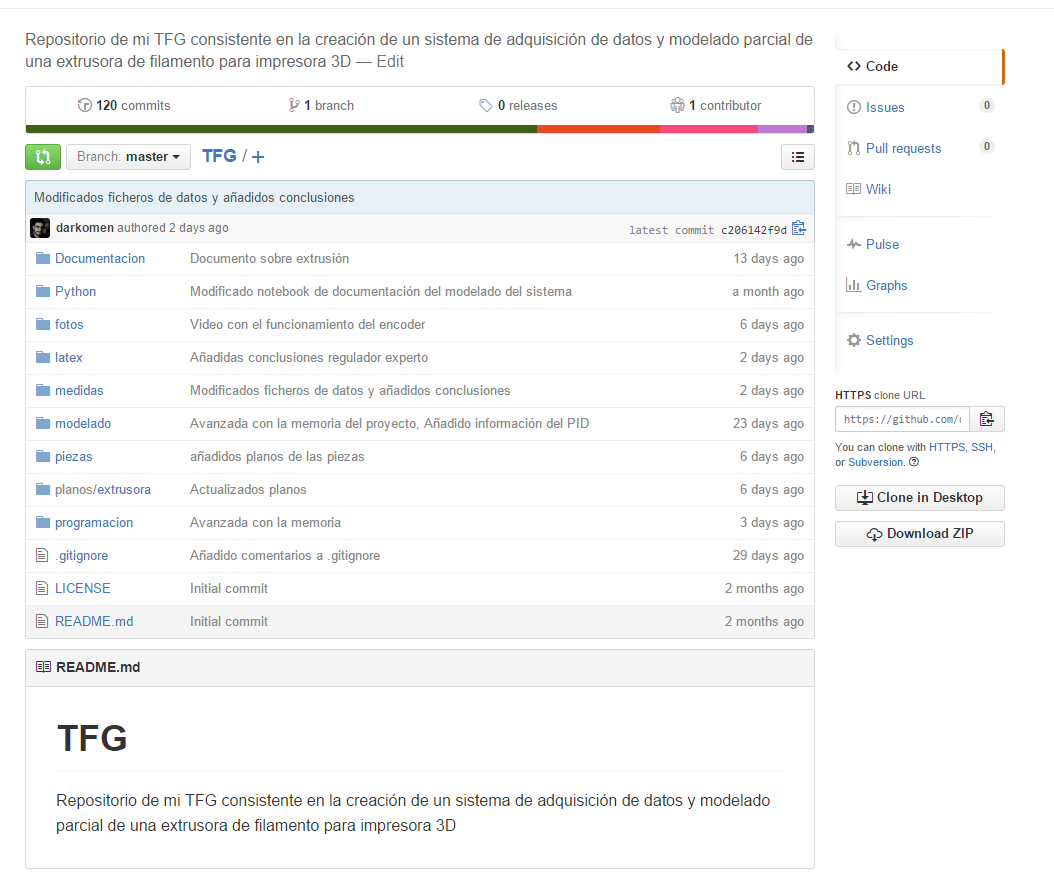
\includegraphics[width=0.65\textwidth]{images/github.png}
    \caption[Repositorio online del proyecto.]{Repositorio  en el que todos los ficheros usados para la realización del mismo están disponibles online}
    \label{fig:github}
\end{figure}

\subsection{IPython Notebook}
IPython Notebook añade funcionalidades extra a Python, como puede ser resaltado de líneas, coloreado de sintaxis, autocompletado entre otras ventajas. Además ofrece la posibilidad de combinar ejecución de código python, mostrar texto matemático, gráficas y contenido múltimedia \cite{ipython}. Podemos ver un ejemplo en la Figura \ref{fig:ipython}

\begin{figure}[H]
    \centering
    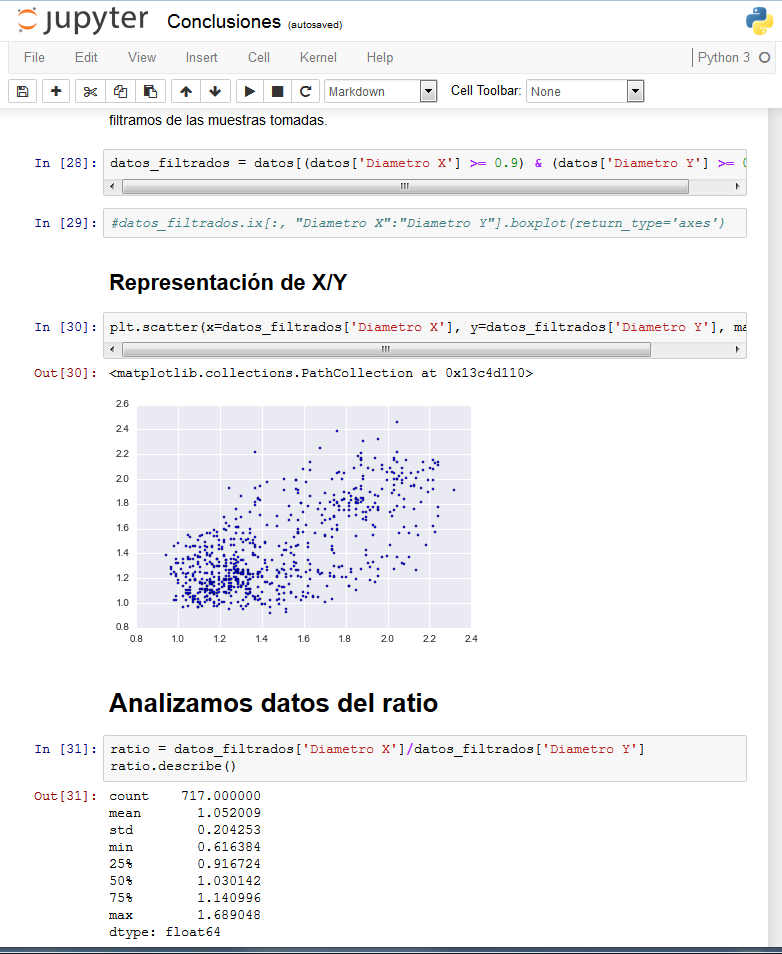
\includegraphics[width=0.5\textwidth]{images/ipython.png}
    \caption[Ejemplo de iPython Notebook usado en el proyecto.]{Ejemplo de iPython Notebook usado en el proyecto. En la Figura vemos, como se puede combinar texto plano, ejecución de código Python y mostrar gráficas}
    \label{fig:ipython}
\end{figure}

Esta herramienta se ha utilizado en el proyecto para poder calcular el modelo matemático de un sistema e implementar un regulador PID, así mismo, se han analizado los datos adquiridos durante una producción de filamento y comprobar los resultados del sistema diseñado. Los cuadernos realizados están disponibles para su consulta y descarga en el repositorio que se ha creado para el proyecto \cite{githubTFG}.

\subsection{GNU Octave}
GNU Octave es un programa libre para realizar cálculos numéricos. Ofrece un interprete de comandos, donde se van escribiendo los comandos que queramos realizar. También permite mostrar gráficas con una serie de datos numércios. Se le considera el equivalente a Matlab \cite{octave}. Esta herramienta se ha utilizado en el proyecto para calcular el modelo matemático de un sistema, para la posterior implementación de un regulador PID.

\subsection{Autodesk Inventor}
Durante la ejecución del proyecto, ha sido necesario realizar piezas específicas a nuestras necesidades. Para ello se han usado impresoras 3D y diseñado las propias piezas que en cada momento han sido necesarias. El diseño de las mismas ha sido realizado en la herramienta Autodesk Inventor. Esta herramienta ofrece un paquete de modelado de sólidos en 3D profesional que compite con otros programas de diseño asistido por ordenador, como pueden ser Catia, Pro/ENGINEER y Solid Edge entre otros.

\begin{figure}[H]
    \centering
    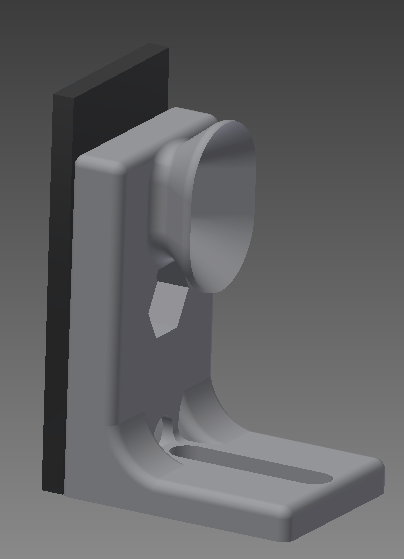
\includegraphics[width=0.25\textwidth]{images/peletizadora/guia.png}
    \caption[Ejemplo de pieza diseñada con Autodesk Inventor.]{Ejemplo de pieza diseñada con Autodesk Inventor. En la Figura vemos una pieza específica diseñada para el proyecto.}
    \label{fig:pieza}
\end{figure}

\subsection{Software de impresión 3D}
Para la fabricación de las piezas diseñadas, se han usado impresoras Witbox y un software capaz de laminar el fichero STL en G-code para que la impresión de la pieza sea correcta. En este software es donde se conFiguran los parámetros de fabricación final de la pieza.

\begin{figure}[H]
    \centering
    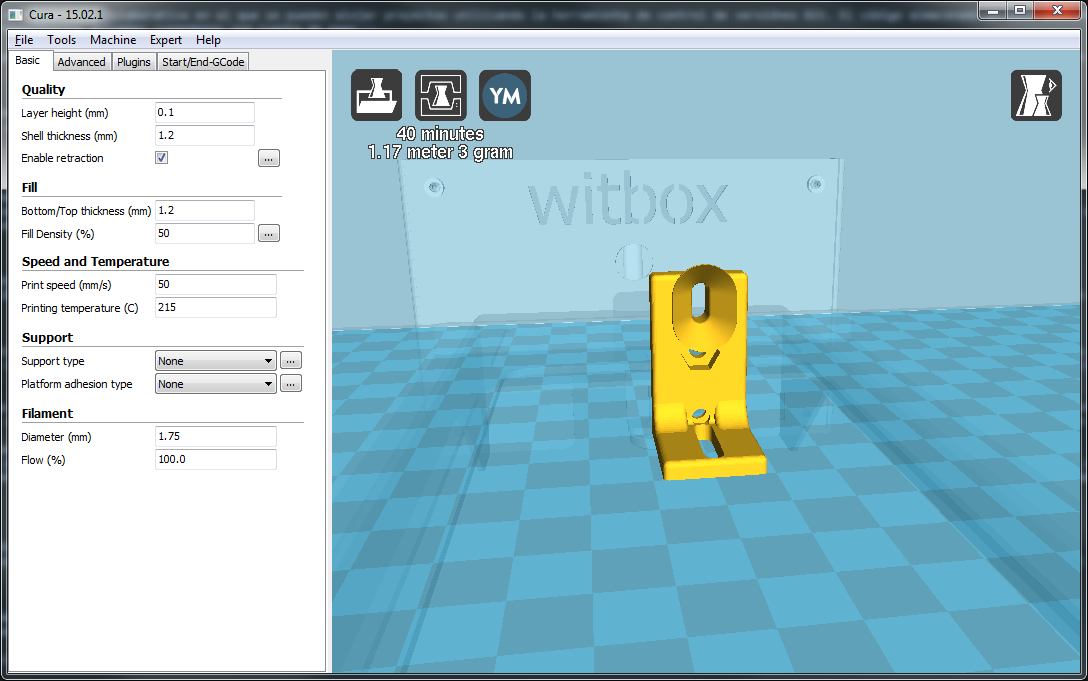
\includegraphics[width=0.7\textwidth]{images/cura.png}
    \caption[Pieza diseñada abierta en cura.]{Pieza diseñada abierta en cura. Podemos ver como en el laminador se pueden conFigurar los distintos parámetros de fabricación de la pieza.}
    \label{fig:cura}
\end{figure}


\section{Elección de los componentes.}

Se quiere desarrollar un sistema capaz de leer información de varios sensores y dado el caso activar elementos de control, todos ellos situados en un entorno industrial como es una fábrica de extrusión de polímeros. Por ello, el sistema elegido debe ser lo más robusto posible y tener capacidades de expansión por módulos para que, según la línea en la que se instale, se pueda acceder a una gran variedad de sensores.\\ 

Así mismo, el sistema debe tener la posibilidad de almacenar información en una memoria externa, ya sea, alojada dentro del mismo sistema o en un sistema externo, como puede ser un servidor de bases de datos. También, debe poder estar conectado a una red ethernet con acceso a Internet, para poder acceder de forma remota desde fuera de la fábrica.\\ 

Debido a todas estas características, se decide usar como unidad central del sistema, un autómata programable industrial (PLC) que en una primera aproximación parece ser lo más adecuado. También se intenta buscar un PLC que nos ofrezca las siguientes ventajas, no siendo estas imprescindibles, pero si ayudarán a la hora de elegir un modelo u otro:

\begin{itemize}
		\item{Licencia de desarrollo libre.}
		\item{Modelo básico con el mayor número de especificaciones necesarias.}
		\item{Capacidad de expansión de las características por medio de módulos.}
\end{itemize}

De este modo, conseguimos reducir el coste total del proyecto. Partiendo de estos requisitos y buscando distintos proveedores por Internet, las empresas que mejor se ajustan son:

\begin{itemize}
		\item{\textbf{UNITRONICS:} La compañía ofrece un PLC con pantalla HMI de bajo coste, que es idóneo para pequeños proyectos que no requieran demasiada capacidad. El principal problema es que no dispone de ninguna expansión para almacenar en tarjetas SD, ni se tiene conocimiento de que se pueda conectar a una base de datos MYSQL de forma directa.}
		\item{\textbf{WAGO:} Cumple todos los requisitos que necesitamos, sin embargo, es necesario pagar una licencia para poder usar el software disponible}
		\item{\textbf{ABB:} El PLC de la gama eco trae de serie la mayoría de las cosas que necesitamos, además, si no se superan ciertas limitaciones, no es necesario pagar una licencia para poder usar el software de desarrollo.}
\end{itemize}

Se habla con cada uno de los distribuidores que ofrecen los productos en España, pidiendo un presupuesto con el material necesario para suplir las necesidades del proyecto como vemos en la tabla \ref{tab:presupuestos}

\begin{table}[H]
	\centering
	\begin{tabular}{cc}
		{\bf Distribuidor} & {\bf Precio (\euro{})} \\ \hline
		Unitronics         & 390              \\
		Wago               & 1374             \\
		Abb                & 506              \\
	\end{tabular}
	\caption[Presupuesto de los tres distribuidores]{Presupuestos de los tres distribuidores. Se ve la gran diferencia de precios entre los distintos distribuidores.}
	\label{tab:presupuestos}
\end{table}

Debido al alto presupuesto que propone Wago se descarta ya que el precio de ABB es muy competitivo. De hecho es la marca que se elije, puesto que en comparación el coste con la marca Unitronics no supone un gasto excesivo y la fiabilidad de los autómatas y el software que provee ABB es mejor.\\

Una vez adquirido el PLC lo siguiente será realizar el montaje del armario donde irá colocado en la fábrica. En el anexo \ref{ane:plc} se detalla el proceso de construcción que se ha llevado acabo.\\

Se mantienen conversaciones con los responsables de PESL para poner en común cuales son los dispositivos que disponen en la fábrica, sin embargo, se muestran reticentes al proyecto y no nos dan acceso a su extrusora para poder realizar el proyecto.\\

A pesar de ello, no supone un problema para la realización del proyecto, ya que puede realizarse sin tener ninguno de los materiales, unicamente con el PLC y simuladores software podríamos realizarlo, pero no podríamos demostrar que nuestro sistema es útil. En el departamento de robótica e innovación de BQ se dispone de un KIT DIY de una extrusora de filamento, filastruder.\\

    \begin{figure}[H]
            \centering
            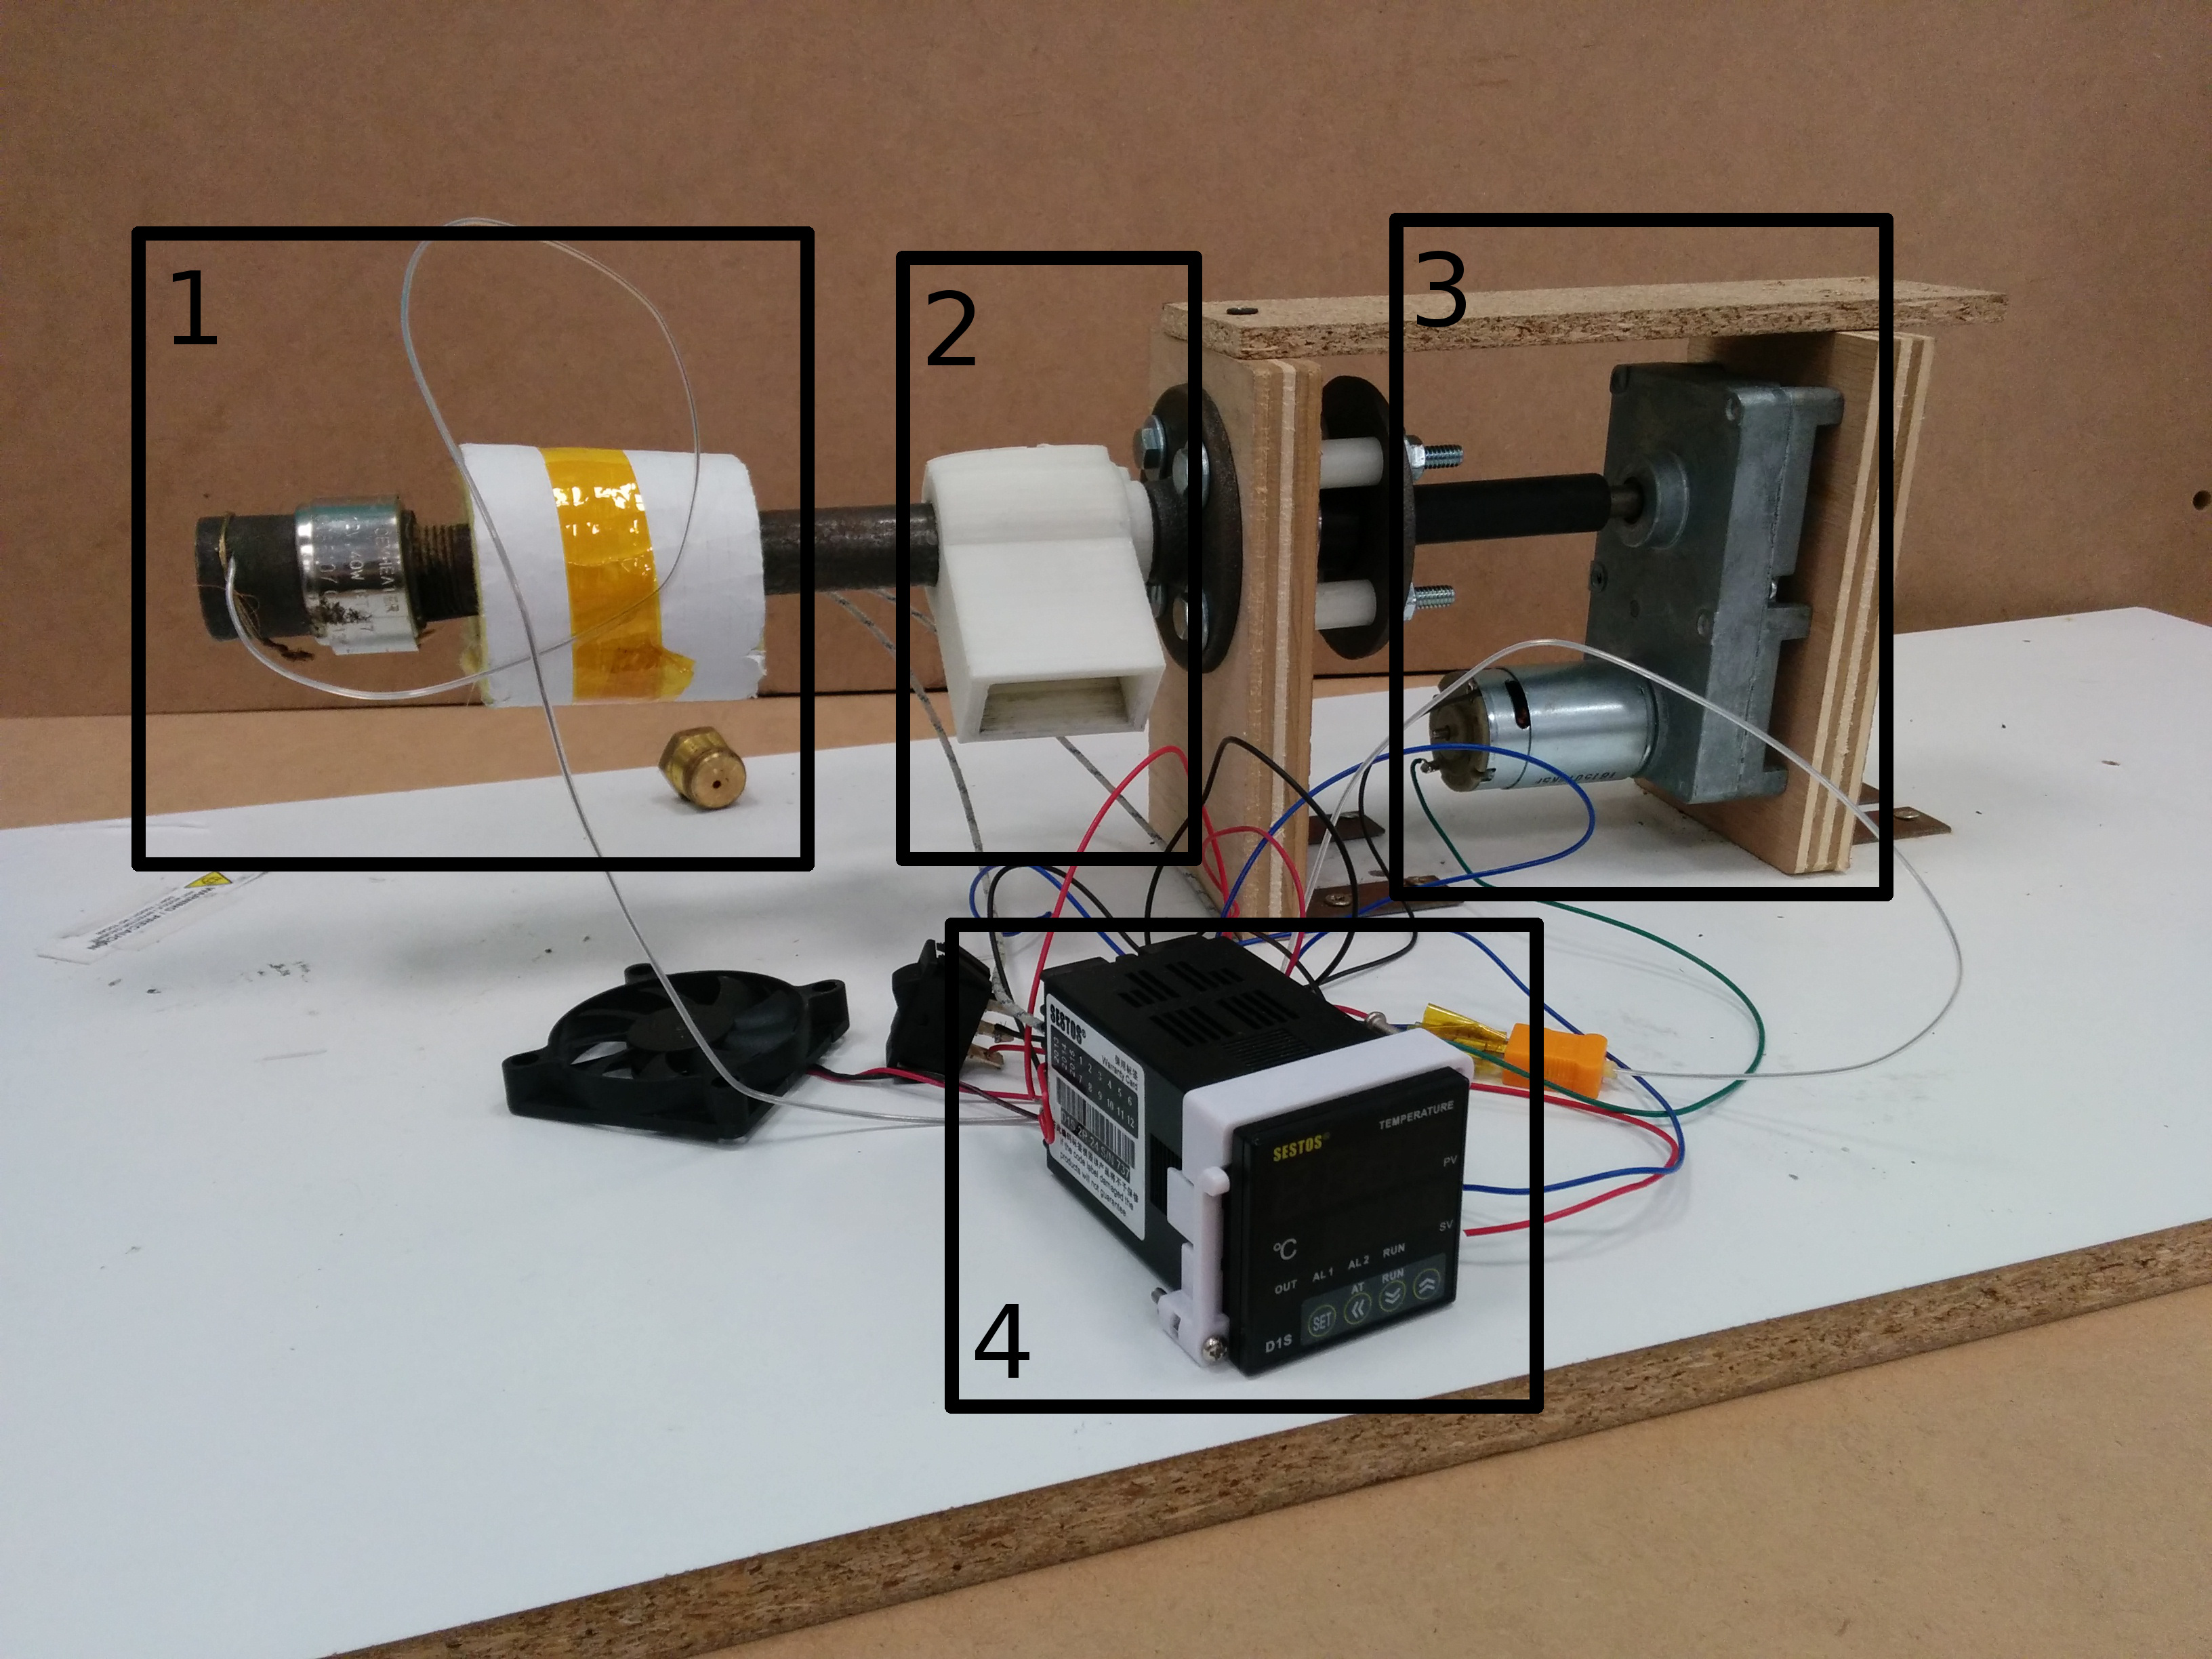
\includegraphics[width=0.6\textwidth]{images/filaextruder/IMG_20150313_11163.jpg}
            \caption[Maqueta de filastruder montada]{Maqueta de filastruder montada. (1) Boquilla y calefactor de la extrusora. (2) Tolva de alimentación de material. (3) Motor para mover el husillo. (4) Controlador de temperatura.}
            \label{fig:hardware_filastruder}
    \end{figure}

Filastruder se presenta como proyecto en Noviembre de 2012 \cite{filastruder} y consiguió recaudar $212.278 \$$ en una campaña de crowfunding en kickstarter\footnote{https://www.kickstarter.com/projects/833191773/filastruder-a-robust-inexpensive-filament-extruder?lang=es}. Es un extrusor de baja capacidad y de bajo coste, liberado como Open Source. Todo el proceso de construcción del extrusor se documentó en el foro y se creó una comunidad de usuarios interesados en los extrusores caseros.\\

Algunas de las características de este extrusor son:

\begin{table}[H]
    \centering

        \begin{tabular}{lc}
        \textbf{Par de detenimiento del motor}            & $12N.m$                           \\
        \textbf{Velocidad del motor}                      & $3 rpm$                           \\
        \textbf{Tiempo para extruir 1kg}                  & $24H$                             \\
        \textbf{Diámetro del husillo}                     & $15.875mm$                        \\
        \textbf{Longitud del husillo}                     & $255mm$                           \\
        \textbf{Tolerancia declarada}                     & $\pm 0.05 mm$                     \\    

    \end{tabular}
    \caption[Características filastruder.]{Características filastruder. Fuente\cite{tfg_diego}}
    \label{tab:caract_filas}
\end{table}

Debido a que la maqueta ha estado almacenada durante años sin usar, el funcionamientor no es el adecuado para crear filamento en condiciones, sin embargo, es completamente útil para la realización del proyecto. Ya que con dos sensores de temperatura, dos cartuchos calefactores y un sensor de diámetro, podremos simular una extrusora industrial, de esta manera también, demostramos que el sistema es totalmente escalable y con cambios en el software podremos adquirir datos de cualquier extrusora. En el anexo \ref{ane:filastruder} se detalla el proceso llevado a cabo para montar la filastruder. \\

Se decide usar un sensor de diámetro opensource del cual, toda la información necesaria para su construcción está accesible via online \cite{thing_filamento}. En el anexo \ref{ane:sensor} se detalla el proceso llevado a cabo para su construcción.\\

A la hora de obtener matería prima para poder extruir filamento, se decide construir una peletizadora para poder reciclar filamento que no cumple las condiciones para ser usado en una impresora 3D (ver anexo \ref{ane:peletizadora}). Antes de extruir el filamento, se comprueba si los pellets reciclados son aptos para la extrusión.\\

Se realizan ensayos por calorimetría diferencial de barrido (DSC). El DSC es una técnica que permite el estudio de las transiciones de fase en los materiales polímeros\cite{DSC1} lo que es de suma importancia a la hora de establecer sus condiciones de procesado y aplicaciones tecnológicas, ya que el tipo de fases y transiciones entre ellas determinan su comportamiento físico macroscópico.\\

Las medidas de DSC se hicieron en un calorímetro TA Instruments Q20 con sistema de enfriamiento y bajo atmósfera de nitrógeno. El aparato se calibró con Indio como sustancia de referencia ($Tm = 156.6 ^o C$, $\delta H = 28.45 J/g$). En el ensayo se sometió al polímero a una fusión a $20 ^o C/min$, seguida de una cristalización y una segunda fusión, a la velocidad de $5 ^o C/min$.\\

Se empleó el calor de fusión del PLA $100\%$ cristalino, 93 J/g. Los errores en la determinación de las temperaturas, en el cálculo de la entalpía y en el de la cristalinidad se estimaron en $\delta1 ^o C$, $\pm4 J/g$ y $\pm0.04$ respectivamente. El peso de las muestras osciló entre 6 y10 mg, y las temperaturas de transición, Tm y Tc se tomaron en el punto máximo de la curva endoterma o exoterma. La Tg se tomó a la temperatura en la que se alcanza la mitad de la diferencia de calor específico existente entre el estado amorfo vítreo y el amorfo elastómero, es decir $T_{g} = 0.5 \pm C_{p}$.\\

Se incluye a continuación los resultados obtenidos en el experimento. En la Figura \ref{fig:analisis_dsc} se observa cómo en condiciones térmicas de temperatura de transición vítrea (Tg) y temperatura de fusión, ambos filamentos son prácticamente iguales. Como vemos en la tabla \ref{tab:dsc2} no ocurre lo mismo con la cristanilidad del polímero, el cual difiere de uno a otro, por que las condiciones de fabricación no son las mismas.\\

\begin{figure}[H]
    \centering
    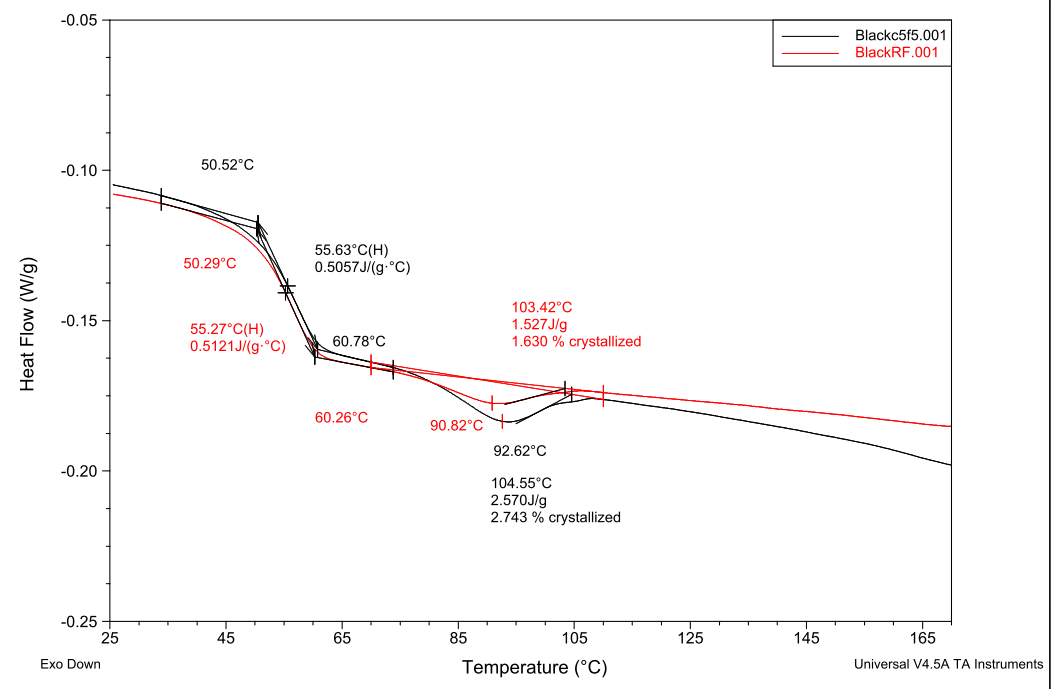
\includegraphics[width=0.9\textwidth]{images/dsc.png}
    \caption[Resultado del análisis con DSC de filamento reciclado.]{Resultado del análisis con DSC de filamento reciclado.En la imagen, vemos el filamento original (color negro) comparado coon el filamento reciclado (color rojo). Podemos llegar a la conclusión de que el filamento reciclado es apto para reutilizar.}
    \label{fig:analisis_dsc}
\end{figure}

En las tablas \ref{tab:dsc1} y \ref{tab:dsc2} podemos ver los datos obtenidos:

\begin{table}[H]
    \centering
    \begin{tabular}{llllll}
        \multicolumn{6}{c}{Glass Transition}                                                        \\
                            & Onset (ºC) & Midpoint (ºC) & End (ºC) & Height W/g & Delta Cp (J/gºC) \\ \hline
        FIlamento Inicial   & 60.78      & 55.63         & 50.52    & 0.04215    & 0.5057           \\
        Filamento reciclado & 60.26      & 55.27         & 50.29    & 0.04268    & 0.5121          
    \end{tabular}
    \caption[Datos del DSC con la transición vítrea del filamento.]{Datos del DSC con la transición vítrea del filamento. En los resultados podemos observar, cómo apenas se produce una degradación en las propiedades térmicas del material reciclado, siendo los valores, muy similares de una muestra a otra}
    \label{tab:dsc1}
\end{table} 


\begin{table}[H]
    \centering
    \begin{tabular}{lllllll}
        \multicolumn{7}{c}{Peak Integration}                                                                                 \\
                            & Start (ºC) & Onset (ºC) & Midpoint (ºC) & Stop (ºC) & Area J/g & Special Area (\% crystalized) \\ \hline
        Filamento Inicial   & 109.99     & 104.55     & 92.62         & 69.98     & 2.570    & 2.743                         \\
        Filamento reciclado & 109.99     & 103.42     & 90.82         & 69.98     & 1.527    & 1.630                        
    \end{tabular}
    \caption[Datos del DSC con la cristanilidad del filamento]{El único dato que difiere de un filamento a otro, es el porcentaje de cristanilidad, y puede ser debido a que ambos filamentos no están fabricado con la misma máquina}
    \label{tab:dsc2}
\end{table}

A falta de realizar un ensayo de propiedades mecánicas de ambos filamentos, podemos dar como válido el pellet reciclado con la peletizadora para su uso en la extrusión del mismo.

\section{Programación del PLC.}

Llegados a este punto, disponemos de todo el material necesario para la realización de una pequeña extrusora de filamento y la adquisición de sus datos más característicos en la producción. El siguiente paso es realizar la programación del PLC.\\

Las acciones que debe realizar el PLC son las siguientes:

\begin{itemize}
    \item{Controlar la temperatura del extrusor.}
    \item{Controlar motor del husillo.}
    \item{Leer información del sensor de diámetro.}
    \item{Almacenar la información tomada en un fichero de datos.}
    \item{Visualizar en una página web el estado de la producción.}
\end{itemize}

Para desarrollar el software que gestione el PLC, se usa una máquina de estados en la que pasando por diversos estados, se irán ejecutando las acciones de control. Debemos entrar en modo producción mediante la activación de una variable. Si estamos en producción, pasaremos por los distintos estados y mientras no estemos en producción, las salidas digitales y valores de consigna de los PID son reseteados a cero como medida de seguridad. Una vez que entremos en producción, el primer paso es inicializar el programa, generamos el nombre del fichero donde almacenamos los datos. Después se genera el fichero CSV y en caso de que no se produzca ningún error, se almacena la cabecera en el fichero CSV, para pasar a la producción como tal. Se controlará la temperatura del dado, se registrarán los valores de diámetros y temperaturas y se irán almacenando en el fichero CSV. El control del motor del husillo se hace de forma manual desde la visualización online.\\

La máquina de estados se muestra en la Figura \ref{fig:plc_estados}

\begin{figure}[H]
    \centering
    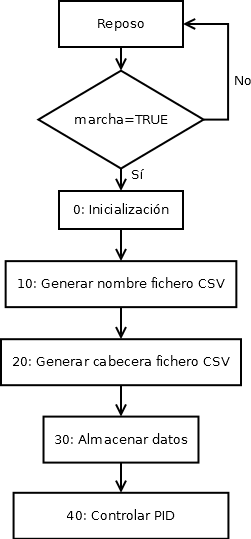
\includegraphics[width=0.25\textwidth]{images/PLC/diagrama.png}
    \caption[Diagrama de estados PLC.]{Diagrama de estados PLC.}
    \label{fig:plc_estados}
\end{figure}

\subsection{Controlar la temperatura del extrusor}
\label{sec:plc_PID}

Se implementa un regulador PID para regular la temperatura del extrusor. Es necesario conocer la planta del sistema que queremos regular para implementar de forma correcta el PID. En nuestro caso el sistema a controlar es el calentamiento del dado, por ello, debemos modelar primeramente el sistema. En la Figura \ref{fig:plc_sistema} podemos ver un esquema de un sistema con un regulador PID\\

\begin{figure}[H]
    \centering
    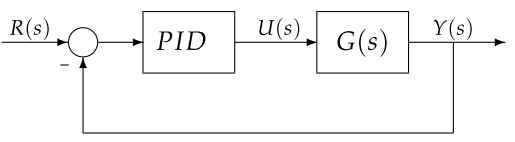
\includegraphics[width=0.4\textwidth]{images/PLC/sistema.png}
    \caption[Sistema con un regulador PID.]{Sistema con un regulador PID. La salida del sistema tendrá una realimentación a la entrada del regulador, para tomar acción de control.}
    \label{fig:plc_sistema}
\end{figure}

Con ayuda del programa que se desarrolla en el PLC haremos las siguientes tareas:

\begin{itemize}
    \item{Registrar temperaturas del dado.}
    \item{Encender de forma controlada la resistencia de calentamiento.}
    \item{Analizar los datos obtenidos.}
\end{itemize}

Analizamos como se comporta el sistema en lazo abierto, sin ningún tipo de control. Partiendo de una temperatura ambiente, se registran los valores de las temperaturas para a continuación encender la resistencia de calentamiento y ver cómo la temperatura va aumentando a medida que pasa el tiempo. Una vez que la temperatura sobrepase un valor que nosotros establezcamos, pararemos el experimento.\\

Con ayuda del lenguaje de programación Python y varias herramientas de análisis de datos como son: IPython, Scipy, Pandas y Numpy, analizamos los datos obtenidos. Las gráficas presentadas a continuación, así como los cálculos están realizadas con estas herramientas.

\begin{figure}[H]
    \centering
    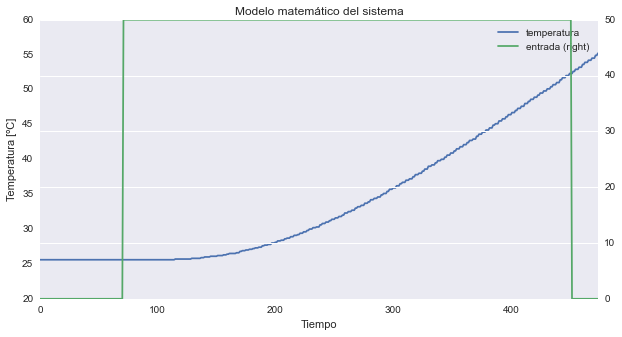
\includegraphics[width=0.75\textwidth]{images/PLC/modelado/modelado_9_1.png}
    \caption[Respuesta del sistema en lazo abierto]{Respuesta del sistema en lazo abierto. Observamos como a medida que avanza el tiempo, también lo hace la temperatura de manera exponencial.}
    \label{fig:plc_lazo_abierto}
\end{figure}

Calcularemos cual es la ecuación que mejor se ajuste a nuestros datos y tendremos el polinomio que caracteriza nuestro sistema.

\begin{figure}[H]
    \centering
    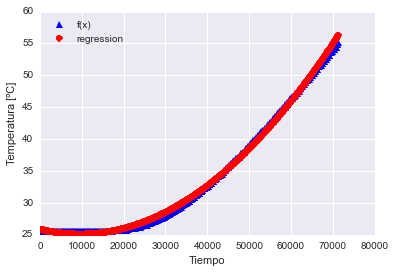
\includegraphics[width=0.5\textwidth]{images/PLC/modelado/modelado_13_1.png}
    \caption[Ajuste de la recta.]{Ajuste de la recta. Calculamos el polinomio que mejor se adapte a nuestros datos.}
    \label{fig:plc_lazo_abierto2}
\end{figure}
$$P_x=  25.9459 -1.5733 \cdot 10^{-4} \cdot X - 8.18174 \cdot 10^{-9} \cdot X^2$$

Si calculamos la transformada de laplace del sistema, obtenemos la planta de nuestro sistema, con la cual podremos implementar el regulador PID:

$$G_s = \frac{25.95 \cdot S^2 - 0.00015733 \cdot S + 1.63635 \cdot 10^{-8}}{S^3}$$

Aplicando el método de sintonizacion de Ziegler-Nichols basado en la curva reacción calcularemos el PID para poder regular correctamente el sistema.Este método consiste en estudiar el sistema en lazo abierto con escalón unitario, calculamos parámetros como la máxima pendiente de la curva y el retardo, y establecemos con ellos las ganancias del controlador PID\cite{PID}. Nos da de manera rápida unos valores de $K_p$, $K_i$ y $K_d$ orientativos, para que podamos ajustar correctamente el controlador. Con ayuda de la herramienta Open Source Octave, calculamos los valores de ganancia que serán los que apliquemos a nuestro regulador.

\Cpp
\begin{lstlisting}
pkg load control
%los datos en la funcion tf() debe ser el numerador y denominador de nuestro sistema.
H=tf([25.95 0.000157333 1.63635E-8],[1 0 0 0]);
step(H);
dt=0.150;
t=0:dt:65;
y=step(H,t);
dy=diff(y)/dt;
[m,p]=max(dy);
yi=y(p);
ti=t(p);
L=ti-yi/m
Tao=(y(end)-yi)/m+ti-L
Kp=1.2*Tao/L
Ti=2*L;
Td=0.5*L;
Ki=Kp/ti;
Kd=Kp*Td;
\end{lstlisting}

En esta primera iteración, los datos obtenidos son los siguientes: $K_p = 6082.6$ $K_i=93.868 K_d=38.9262$. Con lo que nuestro regulador tiene la siguiente ecuación característica:

$$G_s = \frac{38.9262 \cdot S^2 + 6082.6 \cdot S + 93.868}{S}$$

Una vez que tenemos las ganancias de nuestro regulador PID, volvemos a realizar el experimento de calentar la resistencia hasta un valor de temperatura deseado, en este caso 80ºC y vemos cual es la respuesta de nuestro sistema:

\begin{figure}[H]
    \centering
    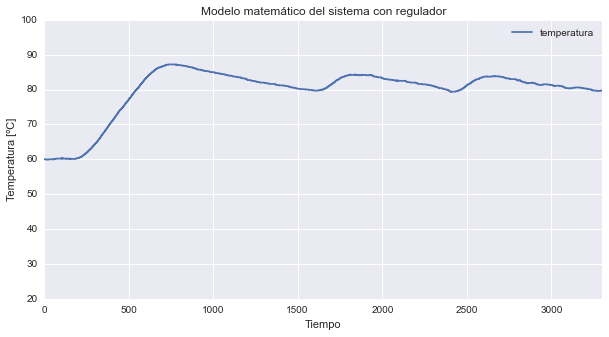
\includegraphics[width=0.75\textwidth]{images/PLC/modelado/modelado_26_1.png}
    \caption[Respuesta del sistema con PID iteracción 1.]{Respuesta del sistema con PID. Primera aproximación para obtener unos valores del regulador adecuados.}
    \label{fig:plc_PID1}
\end{figure}

Como podemos observar en la Figura \ref{fig:plc_PID1} tenemos una sobreoscilación sobre el setpoint elevada:

$$M_{p}=\frac{T_{max}-Setpoint}{Setpoint} \cdot 100 = \frac{87.20-80}{80} \cdot 100 = 9\%$$ 

Siendo el error en régimen  permanente de 3.70.\\

Una vez introducido el controlador, la temperatura tiende a estabilizarse, sin embargo tiene mucha sobreoscilación. Por ello aumentaremos los valores de $K_i$ y $K_d$, siendo los valores de esta segunda iteracción los siguientes:
$K_p = 6082.6$ ,$K_i=103.25$ y $K_d=51.425$\\

Realizando una segunda iteracción en el cálculo de nuestro regulador obtenemos lo siguiente:

\begin{figure}[H]
    \centering
    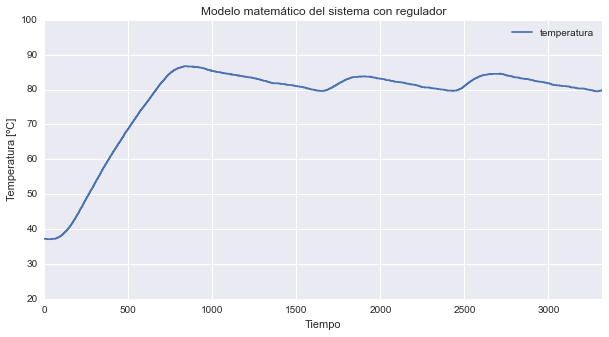
\includegraphics[width=0.75\textwidth]{images/PLC/modelado/modelado_30_1.png}
    \caption[Respuesta del sistema con PID. Iteracción 2]{Respuesta del sistema con PID. Segunda aproximación para obtener unos valores del regulador adecuados.}
    \label{fig:plc_PID2}
\end{figure}

Esta vez los resultados obtenidos son:
$$M_{p}=\frac{T_{max}-Setpoint}{Setpoint} \cdot 100 = \frac{86.70-80}{80} \cdot 100 = 8.38\%$$ 

Siendo el error en régimen permanente de 3.50.\\

En esta segunda iteracción hemos logrado bajar la sobreoscilación inicial, pero tenemos mayor error en regimen permanente. Por ello volvemos a aumentar los valores de $K_i$ y $K_d$ siendo los valores de esta tercera iteracción los siguientes: $K_p = 6082.6$, $K_i=121.64$ y $K_d=60$\\

Realizando una tercera iteracción en el cálculo de nuestro regulador obtenemos lo siguiente:

\begin{figure}[H]
    \centering
    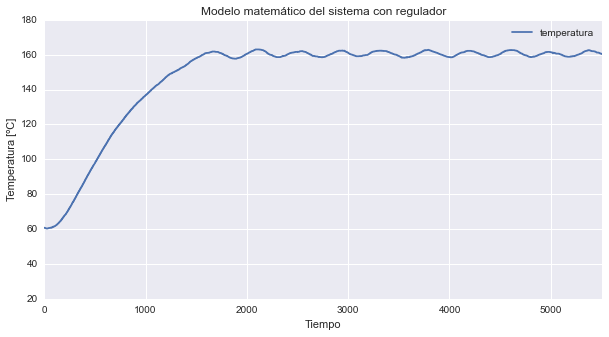
\includegraphics[width=0.75\textwidth]{images/PLC/modelado/modelado_34_1.png}
    \caption[Respuesta del sistema con PID. Iteracción 3]{Respuesta del sistema con PID. Tercera aproximación para obtener unos valores del regulador adecuados.}
    \label{fig:plc_PID3}
\end{figure}

Los resultados obtenidos son:
$$M_{p}=\frac{T_{max}-Setpoint}{Setpoint} \cdot 100 = \frac{163-160}{160} \cdot 100 = 1.88\%$$ 

Siendo el error en régimen permanente de 1.30\\

En este caso, se puso un setpoint de 160ºC. Como vemos, la sobreoscilación inicial ha disminuido en comparación con la anterior iteracción y el error en regimen permanente es menor. Para intentar minimar el error, aumentaremos únicamente el valor de $K_i$. Siendo los valores de esta cuarta iteracción del regulador los siguientes: $K_p = 6082.6$, $K_i=121.64$ y $K_d=150$\\

Realizando una cuarta iteracción en el cálculo de nuestro regulador obtenemos lo siguiente:

\begin{figure}[H]
    \centering
    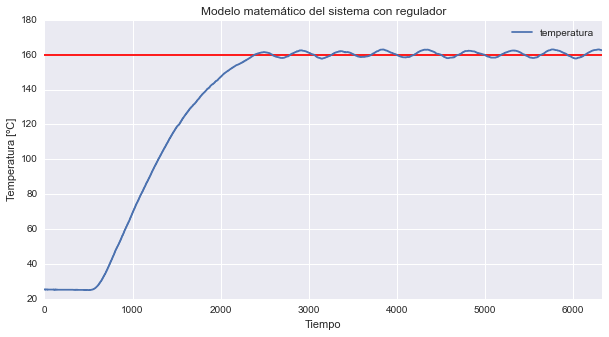
\includegraphics[width=0.75\textwidth]{images/PLC/modelado/modelado_38_1.png}
    \caption[Respuesta del sistema con PID. Iteracción 4]{Respuesta del sistema con PID. Cuarta aproximación para obtener unos valores del regulador adecuados. 4}
    \label{fig:plc_PID4}
\end{figure}

Esta vez los resultados son algo mejores:
$$M_{p}=\frac{T_{max}-Setpoint}{Setpoint} \cdot 100 = \frac{163-160}{160} \cdot 100 = 1.88\%$$ 

Siendo el error en régimen permanente de 1.10\\

Por lo tanto, el regulador que cumple con las especificaciones deseadas tiene la siguiente ecuación característica:
$$G_s = \frac{150 \cdot S^2 + 6082.6 \cdot S + 121.64}{S}$$

\subsection{Leer la información del sensor de diámetro}
\label{sec:plc_diametro}

Los sensores de diámetro están conectados a dos entradas analógicas de tensión del PLC. Será necesario unir la señal de masa (GND) del PLC con la del sensor, para que la referencia al nivel de tensión 0v sea la misma, posteriormente, la salida del sensor de diámetro, se conectará con la entrada analógica del PLC.\\

El PLC convierte el valor de tensión comprendido entre un rango de 0-10V a un valor numérico, a través de un conversor analógico a digital (ADC) de 10bits, es decir, tenemos una resolución de:

$$ \text{Resolución}=\frac{ V_{max} } {2^{10} } = \frac{10}{1024} = 9.76 mV$$

En la ayuda que ofrece el programa de ABB, se observan los valores que asigna el ADC:

\begin{table}[H]
    \centering
    \begin{tabular}{|c|c|c|}
        \hline
        {\bf Intervalo}                   & {\bf 0 ... 10V}                                                   & \multicolumn{1}{l|}{{\bf Valor digital}}                       \\ \hline
        Desbordamiento                    & \textgreater 11.7589                                              & 32767                                                         \\ \hline
        Valor de medición desmasiado alto & \begin{tabular}[c]{@{}c@{}}11.7589\\ .\\ .\\ 10.0004\end{tabular} & \begin{tabular}[c]{@{}c@{}}32511\\ .\\ .\\ 27649\end{tabular} \\ \hline
        Intervalo normal                  & \begin{tabular}[c]{@{}c@{}}10.000\\ .\\ .\\ 0.0004\end{tabular}   & \begin{tabular}[c]{@{}c@{}}27648\\ .\\ .\\ 1\end{tabular}     \\ \hline
    \end{tabular}
    \caption[Valores de conversión del ADC.]{Valores de conversión del conversor analógico a digital. Para un valor de tensión dado, se le asigna un valor decimal.}
    \label{tab:reso_adc}
\end{table}

Se va a trabajar con el rango de intervalo normal. Para poder saber el diámetro que está dando el sensor, se debe leer la entrada analógica y convertir el valor décimal a un valor de tensión, es decir, convertir el valor digital a analogico (DAC), para ello, con los valores del intervalo normal de la tabla \ref{tab:reso_adc} se calcula la ecuación de la recta que lo caracteriza que en este caso es: $Y=3.6168 \cdot 10^{-4} \cdot X$ (ver Figura \ref{fig:plc_DAC})

\begin{figure}[H]
    \centering
    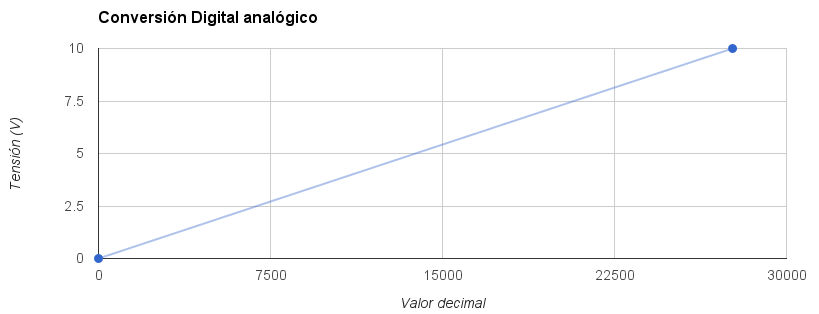
\includegraphics[width=0.75\textwidth]{images/PLC/image.png}
    \caption[Ecuación característica del ADC.]{Ecuación característica del ADC. Con esta ecuación, podemos convertir el valor de tensión a un valor de diámetro.} 
    \label{fig:plc_DAC}
\end{figure}

Con este valor se puede tener acceso al valor del diámetro que tiene el filamento. El siguiente paso entonces, será realizar el almacenamiento de los datos de la producción en un fichero para su posterior análisis.

\subsection{Almacenar la información registrada}
\label{sec:plc_SD}

Se elije un nombre de fichero en el que se usa año, mes, día y minuto para identificar la producción, es decir, tiene un formato \textit{YYMMDDmm.CSV}. El formato elegido para almacenar la información es el de valores separados por coma (CSV). El motivo por el cual se elije este formato es debido a su estandarización y que almacena los datos de forma tabular en texto plano. Gracias a esto, se puede abrir el fichero CSV con cualquier editor de texto y otros programas de hojas de cálculo, para el posterior análisis de los datos, que es uno de los objetivos del proyecto. Por lo tanto, el formato CSV es el idóneo para poder trabajar en el futuro con los datos almacenados.\\

En el progama del PLC se genera una cabecera del fichero CSV, que es la primera fila del fichero, en donde indicará la información que contiene cada columna. La información almacenada en el fichero CSV es la siguiente:

\begin{itemize}
    \item{\textbf{Time Stamp: }Es una secuencia de caracteres en las que se indican hora y fecha de un evento ocurrido. Se almacena con el formato YY-MM-DD HH:MM:SS. Con esta información podremos tener una trazabilidad del filamento almacenado y en caso de producirse un error, ver el momento concreto del mismo.}
    \item{\textbf{Temperaturas: }Valores con las temperaturas del dado y el husillo en la zona de alimentación. De esta manera se comprueba que la temperatura no sufre algún cambio drástico durante el proceso, que puede ser causante de un problema en la calidad final del filamento.}
    \item{\textbf{Diámetros: }Se almacenan los diámetros medidos por el sensor. En este caso se van a poner dos sensores de diámetro para hacer una medición en los dos ejes del filamento.}
    \item{\textbf{Información varia: }Se puede almacenar cualquier información que nosotros deseemos en un futuro (X e Y).}
\end{itemize}

En la tabla \ref{tab:plc_csv} se ve un ejemplo de los datos almacenados en un fichero csv:

\begin{table}[H]
    \centering
    \begin{tabular}{ccccc}
        {\bf time}         & {\bf Tmp Husillo} & {\bf Tmp Nozzle} & {\bf Diámetro X} & {\bf Diámetro Y} \\ \hline
        2015-8-13 11:11:1  & 67.5              & 150.4            & 1.71         & 1.49         \\
        2015-8-13 11:11:2  & 67.5              & 150.4            & 1.82         & 1.51         \\
        2015-8-13 11:11:4  & 67.5              & 150.5            & 1.91         & 1.52         \\
        2015-8-13 11:11:5  & 67.4              & 150.5            & 1.94         & 1.55         \\
        2015-8-13 11:11:7  & 67.4              & 150.5            & 1.91         & 1.56         \\
        2015-8-13 11:11:9  & 67.4              & 150.6            & 1.92         & 1.58         \\
        2015-8-13 11:11:10 & 67.4              & 150.6            & 1.97         & 1.71         \\
        2015-8-13 11:11:12 & 67.4              & 150.6            & 2.02         & 1.89        \\
                -          &    -              & -                & -                & -
    \end{tabular}
    \caption[Muestra de un fichero CSV con datos de producción.]{Muestra de un fichero CSV con datos de producción. Están registrados los datos más importantes de la producción como son. Time Stamp, Temperaturas y Diámetros.}
    \label{tab:plc_csv}
\end{table}

La información se almacena en la tarjeta SD interna del PLC y para poder acceder a ella, se usa un servidor de transferencia de ficheros (servidor FTP) con el que se transfieren ficheros desde el PLC al ordenador mediante una conexión de red, de esta manera, se accede a la SD de forma remota, sin tener que sacar la SD del PLC. Para ello,como se muestra en la Figura \ref{fig:plc_servicios}, se usa el servidor FTP que facilita la herramienta de ABB\\

\begin{figure}[H]
    \centering
    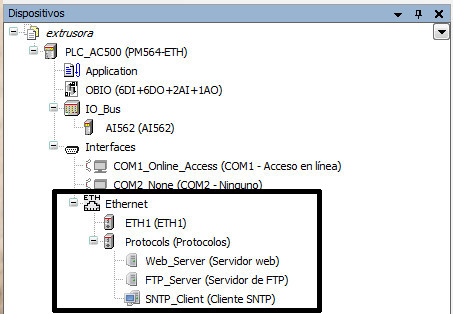
\includegraphics[width=0.5\textwidth]{images/PLC/servicios_plc.jpg}
    \caption[Distintos servicios que dispone el PLC]{Distintos servicios que dispone el PLC. Se pueden instalar distintos servicios de red al PLC: Http, FTP y NTP:}
    \label{fig:plc_servicios}
\end{figure}

En el ordenador, con ayuda de un software cliente FTP se accede aa la IP del PLC que se encuentra en la misma red y se descarga el fichero csv para su posterior estudio (ver Figura \ref{fig:plc_cliente_ftp}).

\begin{figure}[H]
    \centering
    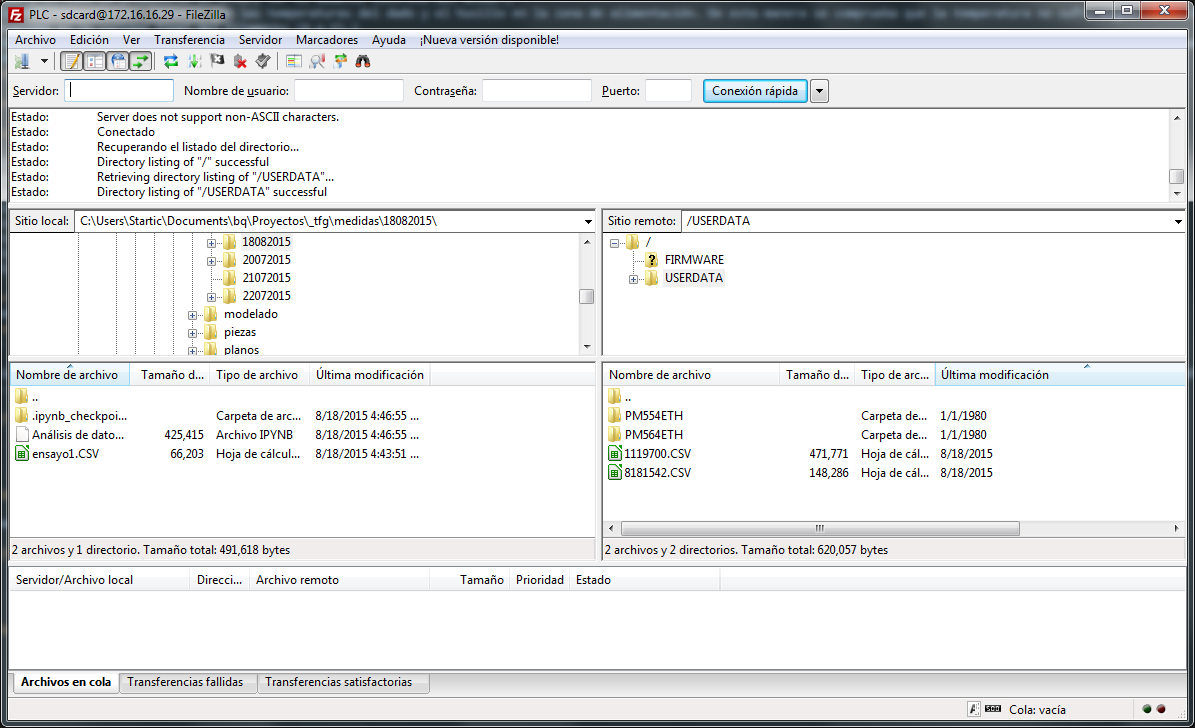
\includegraphics[width=0.95\textwidth]{images/PLC/cliente_ftp.png}
    \caption[Cliente FTP.]{Cliente FTP. Con ayuda de este software, nos podremos conectar a servidores FTP para acceder a los ficheros que hay en el mismo.}
    \label{fig:plc_cliente_ftp}
\end{figure}

\subsection{Visualización web de la producción}
\label{sec:plc_scada}

Para poder visualizar el estado de la producción, se usa una herramienta que incorpora de serie el programa de Abb al igual que el servidor FTP que se vió anteriormente. Esta herramienta, provee un servidor de páginas WEB (ver Figura \ref{fig:plc_servicios}) en la que se puede acceder al estado de variables del programa y se pueden añadir gráficos (ver Figura \ref{fig:plc_visu_web}) que simulen físicamente la planta. Desde esta visualización web se puede:

\begin{itemize}
    \item {Ver temperaturas de Husillo y Dado.}
    \item {Iniciar y parar producción.}
    \item {Controlar marcha del motor del husillo.}
    \item {Ver ruta del fichero en el que se almacenará la información.}
\end{itemize}

\begin{figure}[H]
    \centering
    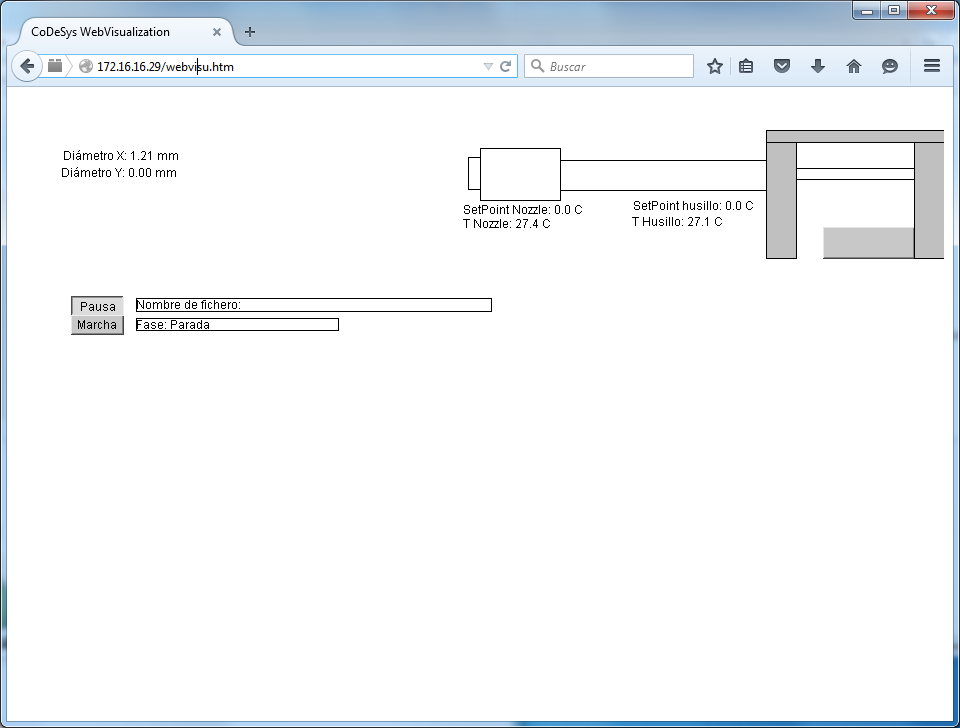
\includegraphics[width=0.95\textwidth]{images/PLC/visu_online.png}
    \caption[Visualización online del sistema.]{Visualización online del sistema.Desde una página web, tenemos acceso a las variables que controlan el proceso.}
    \label{fig:plc_visu_web}
\end{figure}

